
%==========================================================================================
\section{Ressourcenbeschränkte Projektplanung und Zusatzkapazitäten}

\begin{frame}[noframenumbering]
\frametitle{Gliederung}
\tableofcontents[current, hideallsubsections]
\end{frame}

\begin{frame}[t]
\frametitle{Ressourcenbeschränkte Projektplanung}
\begin{center}
\includegraphics[page=3, width=\textwidth]{images/rcpsp.pdf}\\
\end{center}

{\small
Projektdauerminimale Einplanung von Arbeitsgängen $j$ mit gegebenen
\begin{itemize}
\itemsep0em
\item Dauern $d_j$
\item Ressourcenbelastungen $k_{jr}$
\item Reihenfolgebeziehungen $i \in \mathcal{P}_j$
\item Kapazitätsrestriktionen $K_r$
\end{itemize}
}
\end{frame}

%==========================================================================================

\begin{frame}
\frametitle{Projektdauer und Deckungsbeitrag}
\begin{small}
Praxisbeispiel: Aufarbeitung eines Triebwerks durch Dienstleister
\begin{itemize}
\item Projektdauer {\large $\downarrow$} $\implies$ Zahlungsbereitschaft {\large $\uparrow$\\}
\item Überstunden {\large $\uparrow$} $\implies$ Projektdauer {\large $\downarrow$} Kosten {\large $\uparrow$}\\
\item[] \begin{tabbing}
$\Rightarrow$ \= Maximierung des Deckungsbeitrags als Trade-off zwischen\\
\>Dauer- und Kostenminimierung
\end{tabbing}

\end{itemize}
\end{small}
\begin{center}
\includegraphics[page=3,scale=0.29]{images/ErloesKostenDeckungsbeitrag.pdf}
\end{center}
\end{frame}

%==========================================================================================

\begin{frame}[t]
	\frametitle{Projektplanung mit Zusatzkapazitäten}
	\begin{center}
		\includegraphics[width=\textwidth]{images/RCPSPOCIntro.pdf}\\
	\end{center}
	
	{\small
		Deckungsbeitragsmaximale Einplanung von Arbeitsgängen mit zusätzlich gegebenen
		\begin{itemize}
			\itemsep0em
			\item Zusatzkapazitätskostensätzen $\kappa_r$			
			\item Oberen Schranken für Zusatzkapazität $\overline{z}_r$
			\item Projektdauerabhängigen Erlösen $u_t$
		\end{itemize}
	}
\end{frame}

%%%%%%%%%%%%%%%%%%%%%%%%%%%%%%%%%%%%%%%%%%%%%%%%%%%%%%%%%%%%%%%%%%%%%%%%%%%%%%%%%%%%%%%%%%%%%%%%%%%%%%%%%

\section{Heuristische Lösungsverfahren}

\begin{frame}[noframenumbering]
\frametitle{Gliederung}
\tableofcontents[current,currentsubsection]
\end{frame}

\begin{frame}
\frametitle{Genetische Algorithmen}
Repräsentationen im Überblick
\begin{itemize}
	\item \small{Startzeit zwischen Reihenfolge- und Ressourcenzulässigkeit}\\[2mm]
	\begin{small}
	\begin{tabular}{cp{7.5cm}}
	\hline
	Individuum & Planerzeugung\\
	\hline
	$(\lambda)$ & Vervollständigung jeder Alternative ohne ZK\\	
	$(\lambda|\tau)$& Startzeit beliebig in Zeitfenster\\
	$(\lambda|\beta)$& Startzeit an Zeitfensterrand\\
	\end{tabular}
	\end{small}\\[4mm]
	
	\item \small{Vorbestimmung des Ressourcenprofils}\\[2mm]
	\begin{small}
		\begin{tabular}{cp{7.5cm}}
			\hline
			Individuum & Planerzeugung\\
			\hline
			$(\lambda|\tilde{z}_{rt})$ & Kapazität entspricht $K_r+z_{rt}$ mit $z_{rt} \leq \tilde{z}_{rt}$ \\
			$(\lambda|\tilde{z}_r)$ & Kapazität entspricht $K_r+z_r$ mit $z_{rt} \leq \tilde{z}_{r}$\\
		\end{tabular}
	\end{small}
\end{itemize}
\end{frame}

%%%%%%%%%%%%%%%%%%%%%%%%%%%%%%%%%%%%%%%%%%%%%%%%%%%%%%%%%%%%%%%%%%%%%%%%%%%%%%%%%%%%%%%%%%%%%%%%%%%%%%%

\subsection{Vervollständigung ohne ZK $(\lambda)$}
\begin{frame}[noframenumbering]
	\frametitle{Gliederung}
	\tableofcontents[currentsubsection]
\end{frame}

\begin{frame}[t]
	\frametitle{Planerzeugung $(\lambda)$: Einplanung AG 2}
	\begin{center}
		\includegraphics<1>[page=1, scale=0.65]{images/ssgsoc.pdf}
		\includegraphics<2>[page=2, scale=0.65]{images/ssgsoc.pdf}
		\includegraphics<3>[page=3, scale=0.65]{images/ssgsoc.pdf}
		\includegraphics<4>[page=4, scale=0.65]{images/ssgsoc.pdf}
		\includegraphics<5>[page=5, scale=0.65]{images/ssgsoc.pdf}
		\includegraphics<6>[page=6, scale=0.65]{images/ssgsoc.pdf}
		\includegraphics<7>[page=5, scale=0.65]{images/ssgsoc.pdf}\\
		
		\only<1>{
			Bisher Arbeitsgang 1 eingeplant.
			\vspace*{12.5mm}
		}
		
		\only<2>{
			Früheste Reihenfolgezulässigkeit $\underline{t}$\\
			AG 2 mit $ST_2=\underline{t}=1$ einplanen.
			%\vspace*{15mm}
			\textcolor{white}{$\mbox{DB} = u_{8}-\sum_r \sum_t \kappa_r\mbox{z}_{rt} = 1\mbox{ GE} - 4\mbox{ GE} = 3\mbox{ GE}$}
		}
		
		\only<3>{
			Früheste Reihenfolgezulässigkeit $\underline{t}$\\
			AG 2 mit $ST_2=\underline{t}=1$ einplanen.\\
			$\mbox{DB} = u_{8}-\sum_r \sum_t \kappa_r z_{rt} = 1\mbox{ GE} - 1\mbox{ GE} = 0\mbox{ GE}$
		}
		
		\only<4>{
			Inkrementiere\\
			AG 2 mit $ST_2=2$ einplanen.\\
			$\mbox{DB} = u_{8}-\sum_r \sum_t \kappa_r z_{rt} = 1\mbox{ GE} - 1\mbox{ GE} = 0\mbox{ GE}$
		}
		
		\only<5>{
			Inkrementiere\\
			AG 2 mit $ST_2=3$ einplanen.\\
			$\mbox{DB} = u_{9}-\sum_r \sum_t \kappa_r z_{rt} = 0{,}75\mbox{ GE} - 0{,}5\mbox{ GE} = 0{,}25\mbox{ GE}$
		}
		
		\only<6>{
			Früheste Ressourcenzulässigkeit $\overline{t}$\\
			AG 2 mit $ST_4=\overline{t}=4$ einplanen.\\
			$\mbox{DB} = u_{10}-\sum_r \sum_t \kappa_r z_{rt} = 0\mbox{ GE} - 0\mbox{ GE} = 0\mbox{ GE}$
		}
		
		\only<7>{
			Bester Kandidat für Einplanungszeitpunkt\\
			AG 2 mit $ST_4=3$ einplanen.\\
			$\mbox{DB} = u_{10}-\sum_r \sum_t \kappa_r z_{rt} = 0{,}75\mbox{ GE} - 0{,}5\mbox{ GE} = 0{,}25\mbox{ GE}$
		}
	\end{center}
\end{frame}

\begin{frame}
	\frametitle{Genetischer Algorithmus $(\lambda)$}
	\begin{small}
		\begin{center}
			\begin{tabular}{rl}
				\hline 
				Individuum & $(\lambda)=(0,1,4,2,5,3,6,7)$\parbox[c][40pt][c]{0pt}{}\tabularnewline
				\hline 
				Initialpopulation & Regret-Based Biased Random Sampling (LFTs)\tabularnewline
				\hline 
				Rekombination & One Point Crossover\tabularnewline
				\hline 
				Mutation & Neighborhood Swap\tabularnewline
				\hline 
				Fitness & Deckungsbeitrag von induziertem Plan\tabularnewline
				\hline 
			\end{tabular}
		\end{center}
	\end{small}
\end{frame}

%%%%%%%%%%%%%%%%%%%%%%%%%%%%%%%%%%%%%%%%%%%%%%%%%%%%%%%%%%%%%%%%%%%%%%%%%%%%%%%%%%%%%%%%%%%%%%%%%%%%%%%

\subsection{Wahl in Zeitfenster $(\lambda|\tau)$}
\begin{frame}[noframenumbering]
	\frametitle{Gliederung}
	\tableofcontents[currentsubsection]
\end{frame}

\begin{frame}[t]
	\frametitle{Planerzeugung $(\lambda|\tau)$: Einplanung von 2}
	\includegraphics<1-2>[page=1, scale=0.7]{images/ssgstau.pdf}
	\includegraphics<3>[page=2, scale=0.7]{images/ssgstau.pdf}
	\only<1>{\[ ST_2 = \overline{t} - [ (\overline{t}-\underline{t}) \cdot \tau ] \]}
	\only<2>{\[ ST_2 = 4 - [ (4-1) \cdot 0{,}3 ] = 4 - [ 0{,}9 ] = 3\]}
	\only<3>{\[ ST_2 = 4 - [ (4-1) \cdot 0{,}9 ] = 4 - [ 2{,}7 ] = 1\]}
\end{frame}

\begin{frame}
	\frametitle{Genetischer Algorithmus $(\lambda|\tau)$}
	\begin{small}
		\begin{center}
			\begin{tabular}{rl}
				\hline 
				Individuum & $\begin{pmatrix}\lambda\\\tau\end{pmatrix}=\begin{pmatrix}0,1,3,5,2,4,6,7\\0,0.3,0.5,0.8,0.9,0.2,0.1,0.2\end{pmatrix}$\parbox[c][40pt][c]{0pt}{}\tabularnewline
				\hline 
				Initialpopulation & $\tau_j=$ Zufallszahl aus $[0, 1) \; \forall j$\tabularnewline
				\hline 
				Rekombination & Gemeinsamer OPC mit $\lambda$\tabularnewline
				\hline 
				Mutation & $\tau_j=$ Zufallszahl aus $[0,1)$ mit $P_{mutate}$\tabularnewline
				\hline 
				Fitness & Deckungsbeitrag von induziertem Plan\tabularnewline
				\hline 
			\end{tabular}
		\end{center}
	\end{small}
\end{frame}

%%%%%%%%%%%%%%%%%%%%%%%%%%%%%%%%%%%%%%%%%%%%%%%%%%%%%%%%%%%%%%%%%%%%%%%%%%%%%%%%%%%%%%%%%%%%%%%%%%%%%%%

\subsection{Zeitfenstergrenzen $(\lambda|\beta)$}
\begin{frame}[noframenumbering]
	\frametitle{Gliederung}
	\tableofcontents[currentsubsection]
\end{frame}

\begin{frame}
	\frametitle{Planerzeugung $(\lambda|\beta)$: \only<1-2>{untere}\only<3-6>{obere} Einplanung}
	
	\includegraphics<1>[page=1, scale=0.75]{images/SSGSbetaLower.pdf}
	\includegraphics<2>[page=2, scale=0.75]{images/SSGSbetaLower.pdf}
		
	\includegraphics<3>[page=1, scale=0.75]{images/SSGSbetaUpper.pdf}
	\includegraphics<4>[page=2, scale=0.75]{images/SSGSbetaUpper.pdf}
	\includegraphics<5>[page=3, scale=0.75]{images/SSGSbetaUpper.pdf}
	\includegraphics<6>[page=4, scale=0.75]{images/SSGSbetaUpper.pdf}
\end{frame}

\begin{frame}
	\frametitle{$(\lambda|\beta)$-Varianten}
	\begin{itemize}
		\item Arbeitsgangzuordnung: AG $j=\lambda_i$ nutzt ZK, gdw.
		\begin{itemize}
			\item $\beta_i=1$ (Listenposition assoziiert)
			\item $\beta_j=1$ (AG-Nummer assoziiert)\\[4mm]
		\end{itemize}
		\item Einplanungsart
		\begin{itemize}
			\item "`von unten"': Nutze erst Normalkapazität
			\item "`von oben"': Nutze erst Überstunden\\[4mm]
		\end{itemize}
		\item Crossover
		\begin{itemize}
			\item Gemeinsamer One Point Crossover
			\item Zwei getrennte One Point Crossovers\\[5mm]
		\end{itemize}
		\item[$\implies$] Insgesamt $2 \cdot 2 \cdot 2 = 8$ unterschiedliche Varianten
	\end{itemize}
\end{frame}

\begin{frame}
	\frametitle{Genetischer Algorithmus $(\lambda|\beta)$}
	\begin{small}
		\begin{center}
			\begin{tabular}{rl}
				\hline 
				Individuum & $\begin{pmatrix}\lambda\\\beta\end{pmatrix}=\begin{pmatrix}0,1,3,5,2,4,6,7\\0,1,1,0,1,0,1,0\end{pmatrix}$\parbox[c][40pt][c]{0pt}{}\tabularnewline
				\hline 
				Initialpopulation & $\beta_i=$ Zufallszahl aus $\{0,1\} \; \forall i \in \mathcal{J}$\tabularnewline
				\hline 
				Rekombination & One Point Crossover\tabularnewline
				\hline 
				Mutation & $\beta_i=\neg \beta_i$ mit $P_{mutate}$\tabularnewline
				\hline 
				Fitness & Deckungsbeitrag von induziertem Plan\tabularnewline
				\hline 
			\end{tabular}
		\end{center}
	\end{small}
\end{frame}

%%%%%%%%%%%%%%%%%%%%%%%%%%%%%%%%%%%%%%%%%%%%%%%%%%%%%%%%%%%%%%%%%%%%%%%%%%%%%%%%%%%%%%%%%%%%%%%%%%%%%%%

\subsection{Ressourcenprofil $(\lambda|z_{rt})$}
\begin{frame}[noframenumbering]
	\frametitle{Gliederung}
	\tableofcontents[currentsubsection]
\end{frame}

\begin{frame}
	\frametitle{Planerzeugung $(\lambda|z_{rt})$: Einplanung von 2}
	\includegraphics<1>[page=1, scale=0.75]{images/SSGSzrt.pdf}
	\includegraphics<2>[page=2, scale=0.75]{images/SSGSzrt.pdf}
\end{frame}

\begin{frame}
	\frametitle{Genetischer Algorithmus $(\lambda|z_{rt})$}
	\begin{small}
		\begin{center}
			\begin{tabular}{rl}
				\hline 
				Individuum & $(\lambda|\tilde{z}_{rt})=(0,1,3,5,2,4,6,7|\begin{pmatrix} 0 & 2 & \ldots\\ \vdots & \ddots \end{pmatrix})$\parbox[c][40pt][c]{0pt}{}\tabularnewline
				\hline 
				Initialpopulation & $\tilde{z}_{rt}=$ Zufallszahl aus $\{0,\ldots,\overline{z}_{r}\}\;\forall r,t$\tabularnewline
				\hline 
				Rekombination & One Point Crossover\tabularnewline
				\hline 
				Mutation & $\tilde{z}_{rt}=$ Zufallszahl aus $\{0, \ldots, \overline{z}_{r}\}$ mit $P_{mutate}$\tabularnewline
				\hline 
				Fitness & Deckungsbeitrag von induziertem Plan\tabularnewline
				\hline 
			\end{tabular}
		\end{center}
	\end{small}
\end{frame}

%%%%%%%%%%%%%%%%%%%%%%%%%%%%%%%%%%%%%%%%%%%%%%%%%%%%%%%%%%%%%%%%%%%%%%%%%%%%%%%%%%%%%%%%%%%%%%%%%%%%%%%

\subsection{Feste Kapazität $(\lambda|z_{r})$}
\begin{frame}[noframenumbering]
	\frametitle{Gliederung}
	\tableofcontents[currentsubsection]
\end{frame}


\begin{frame}
	\frametitle{Planerzeugung $(\lambda|z_{r})$: Einplanung von 2}
	\includegraphics<1>[page=1, scale=0.75]{images/SSGSzr.pdf}
	\includegraphics<2>[page=2, scale=0.75]{images/SSGSzr.pdf}
\end{frame}

\begin{frame}
	\frametitle{Genetischer Algorithmus $(\lambda|z_{r})$}
	\begin{small}
		\begin{center}
			\begin{tabular}{rl}
				\hline 
				Individuum & $(\lambda|\tilde{z}_{r})=(0,1,3,5,2,4,6,7|0,2,2,0,3,0,\ldots)$\parbox[c][40pt][c]{0pt}{}\tabularnewline
				\hline 
				Initialpopulation & $\tilde{z}_{r}=$ Zufallszahl aus $\{0, \ldots, \overline{z}_{r}\} \; \forall r$\tabularnewline
				\hline 
				Rekombination & One Point Crossover\tabularnewline
				\hline 
				Mutation & $\tilde{z}_{r}=$ Zufallszahl aus $\{0, \ldots, \overline{z}_{r}$\} mit $P_{mutate}$\tabularnewline
				\hline 
				Fitness & Deckungsbeitrag von induziertem Plan\tabularnewline
				\hline
			\end{tabular}
		\end{center}
	\end{small}
\end{frame}

%%%%%%%%%%%%%%%%%%%%%%%%%%%%%%%%%%%%%%%%%%%%%%%%%%%%%%%%%%%%%%%%%%%%%%%%%%%%%%%%%%%%%%%%%%%%%%%%%%%%%%%

\section{Numerische Ergebnisse}
\begin{frame}[noframenumbering]
\frametitle{Gliederung}
\tableofcontents[current, hidesubsections]
\end{frame}


\begin{frame}[t]
\frametitle{Numerische Ergebnisse}
\begin{footnotesize}
\textbf{Parameter:} Populationsgröße $=80$, $P_{mutate}=5\%$\\

\begin{center}
	\begin{tabular}{ccc}
		\multicolumn{3}{c}{\textbf{Testinstanzen}}\\
		Datensatz & \#Projekte & Zeitlimit\\
		j30 & 199 & $1s$\\
		j120 & 586 & $15s$
	\end{tabular}
\end{center}

\begin{center}	
\tabcolsep=0.16cm
\begin{tabular}{|c|rrrc|rrrc|}
	\hline
	& \multicolumn{4}{c|}{j30} & \multicolumn{4}{c|}{j120}\\
	 & $\varnothing$ Gap & $\overline{\mbox{Gap}}$ & Opt & $\varnothing$ Rang & $\varnothing$ Gap & $\overline{\mbox{Gap}}$ & BBL & $\varnothing$ Rang \\[3pt]
	\hline
   $(\lambda|z_{rt})$&1.41\%&\textbf{8.83\%}&46.73\%&1.98&1.91\%&12.38\%&21.20\%&3.63\\
	\hline
   $(\lambda|z_r)$&3.01\%&45.00\%&28.64\%&2.60&\textbf{0.95\%}&\textbf{8.30\%}&\textbf{52.14\%}&\textbf{2.19}\\
	\hline
	$(\lambda|\beta)$&2.80\%&45.00\%&29.65\%&2.37&1.61\%&8.31\%&25.98\%&2.97\\
	best & \multicolumn{4}{c|}{AG, Gem. OPC, oberes SGS} & \multicolumn{4}{c|}{Liste, Gem. OPC, unteres SGS}\\
	\hline
	$(\lambda|\beta)$&5.27\%&45.00\%&21.11\%&4.39&11.76\%&28.25\%&8.55\%&9.56\\
	worst & \multicolumn{4}{c|}{Liste, Getr. OPCs, oberes SGS} & \multicolumn{4}{c|}{Liste, Getr. OPCs, oberes SGS}\\
	\hline
	$(\lambda|\tau)$&2.45\%&20.23\%&41.21\%&2.98&4.48\%&14.17\%&2.56\%&6.08\\
	\hline
	$(\lambda)$& \textbf{1.20\%}&14.29\%&\textbf{52.76\%}&\textbf{1.78}&5.04\%&19.18\%&27.52\%&5.40\\
	\hline
\end{tabular}
\end{center}

Deckungsbeiträge $\geq 0$ aufgrund von $u_t$-Definition $\implies$ Rationalskaliert

\end{footnotesize}	

\end{frame}

\section{Ausblick}

\begin{frame}[noframenumbering]
\frametitle{Gliederung}
\tableofcontents[current, hidesubsections]
\end{frame}

\begin{frame}
\frametitle{Ausblick}
\begin{itemize}
\item Verbesserung der Genetischen Algorithmen
	\begin{itemize}
	\item Stellschrauben $N^G$, $N^I$, $P_{mutate}$
	\item Anpassung von Mutation und Crossover\\[6mm]
	\end{itemize}
\item Techniken führender RCPSP-Heuristiken
	\begin{itemize}
	\item Vorwärts-Rückwärts-Verbesserung
	\item Fitnessbasierte Paarbildung und Crossover
	\item Zweite Suchphase in Nachbarschaft\\[6mm]
	\end{itemize}
\item Problemspezifischer B\&B-Algorithmus
\end{itemize}
\end{frame}




